% Declaración responsable de uso de IA — ETSE-UV
\newpage
\thispagestyle{empty}

\vspace*{4mm}
{\centering
\textbf{\large Declaración responsable de uso de Inteligencia Artificial (IA) — ETSE-UV}\\[4pt]
\small Anexo. Modelo de declaración a adjuntar al TFG/TFM entregado por el alumnado.\\[10mm]
}

\newcommand{\formline}[2][8cm]{\underline{\makebox[#1][l]{\small #2}}}

\noindent\textbf{Yo,} \formline[7.5cm]{Carlos Javier Piquer Mañez} \hfill \textbf{con (NIF/NPA)} \formline[3cm]{23874989T}\\[5mm]
\noindent\textbf{Titulación:} \formline[13cm]{Grado en Ingeniería Informática}\\[5mm]
\noindent\textbf{Título del TFG/TFM:} \formline[11.5cm]{Desarrollo de una tienda online para una droguería}\\[7mm]

\noindent\small Declaro que en este trabajo he utilizado las siguientes herramientas de IA (si procede):\\[3mm]

\noindent 1. Herramienta y versión: \formline[11cm]{Claude Code — Claude Sonnet 4.6 (Anthropic, 2025)}\\[2.5mm]
\noindent 2. Herramienta y versión: \formline[11cm]{Google Gemini 2.5 Pro (Google, 2025)}\\[2.5mm]
\noindent 3. Herramienta y versión: \formline[11cm]{}\\[2.5mm]
\noindent 4. Herramienta y versión: \formline[11cm]{}\\[6mm]
\clearpage
% ---- Helpers para casillas ----
\newcommand{\cbox}{$\boxtimes$}  % marcada
\newcommand{\ubox}{$\square$}    % vacía

% ---- Sección 1 ----
\noindent\textbf{1) Dimensiones de uso de la IA} (marca una opción por fila). Determina el grado de uso de la IA en las siguientes dimensiones.

\smallskip
\noindent\small Escala (5 puntos): 1 = No se ha utilizado IA · 2 = Uso muy puntual · 3 = Uso moderado · 4 = Uso frecuente · 5 = Uso intensivo

\smallskip
\renewcommand{\arraystretch}{1.35}
\begin{tabular}{|p{0.66\textwidth}|c|c|c|c|c|}
\hline
\small\textbf{Dimensión} & \small\textbf{1} & \small\textbf{2} & \small\textbf{3} & \small\textbf{4} & \small\textbf{5} \\
\hline
\small Corrección lingüística: ortografía, gramática, puntuación y coherencia formal del texto
& \ubox & \ubox & \ubox & \ubox & \cbox \\
\hline
\small Reescritura y mejora de estilo: reformulación para aumentar claridad, concisión y legibilidad manteniendo el significado
& \ubox & \ubox & \ubox & \cbox & \ubox \\
\hline
\small Síntesis de contenido: elaboración de resúmenes a partir de textos extensos o complejos para identificar ideas clave
& \ubox & \ubox & \cbox & \ubox & \ubox \\
\hline
\small Apoyo en la localización de referencias: propuesta de posibles fuentes (a verificar y citar correctamente)
& \ubox & \ubox & \ubox & \cbox & \ubox \\
\hline
\small Planificación del trabajo: propuesta de esquemas, índices o guiones iniciales para estructurar el documento
& \ubox & \cbox & \ubox & \ubox & \ubox \\
\hline
\small Mejora de la argumentación y la estructura: detección de huecos, redundancias o saltos lógicos y propuesta de reorganización
& \ubox & \ubox & \cbox & \ubox & \ubox \\
\hline
\small Programación (si procede): apoyo en el desarrollo, depuración u optimización de fragmentos de código puntuales
& \ubox & \ubox & \ubox & \cbox & \ubox \\
\hline
\small Programación (si procede): uso generalizado de herramientas de generación de código de forma autónoma a partir de especificaciones
& \ubox & \ubox & \cbox & \ubox & \ubox \\
\hline
\small Análisis de datos (si procede): ayuda exploratoria para limpieza preliminar, generación de hipótesis e identificación de patrones
& \ubox & \ubox & \ubox & \ubox & \cbox \\
\hline
\small Traducción o adaptación lingüística (si procede)
& \cbox & \ubox & \ubox & \ubox & \ubox \\
\hline
\small Soporte en material visual (si procede): ideas para figuras, tablas o gráficos y revisión de su explicación
& \ubox & \ubox & \ubox & \cbox & \ubox \\
\hline
\small Otros (especificar): \underline{\hspace{6cm}}
& \ubox & \ubox & \ubox & \ubox & \ubox \\
\hline
\end{tabular}

\bigskip

% ---- Sección 2 ----
\noindent\textbf{2) Compromisos de uso responsable} (marca tu grado de acuerdo). Determina si se ha realizado un uso responsable de la IA.

\smallskip
\noindent\small Escala (acuerdo): 1 = Totalmente en desacuerdo · 2 = En desacuerdo · 3 = Neutral · 4 = De acuerdo · 5 = Totalmente de acuerdo

\smallskip
\begin{tabular}{|p{0.66\textwidth}|c|c|c|c|c|}
\hline
\small\textbf{Declaración} & \small\textbf{1} & \small\textbf{2} & \small\textbf{3} & \small\textbf{4} & \small\textbf{5} \\
\hline
\small Las ideas principales, interpretaciones y análisis críticos del trabajo son propios.
& \ubox & \ubox & \ubox & \ubox & \cbox \\
\hline
\small El uso de IA no ha sustituido mis competencias básicas de investigación, redacción y razonamiento académico.
& \ubox & \ubox & \ubox & \ubox & \cbox \\
\hline
\small He revisado, contrastado e integrado críticamente cualquier contenido generado con IA antes de incorporarlo.
& \ubox & \ubox & \ubox & \ubox & \cbox \\
\hline
\small He verificado la precisión y fiabilidad del contenido, incluyendo datos, afirmaciones y referencias bibliográficas.
& \ubox & \ubox & \ubox & \cbox & \ubox \\
\hline
\end{tabular}

\bigskip
\clearpage
\noindent\textbf{Observaciones (opcional)}

\smallskip
\noindent\rule{\textwidth}{0.4pt}

\bigskip\bigskip

\noindent\small A través de esta declaración, afirmo que he descrito de manera transparente y fidedigna el uso de IA de este trabajo. Asumo la autoría y responsabilidad de la obra final y confirmo que no he introducido datos personales o confidenciales contraviniendo la normativa de protección de datos personales\footnote{Ley orgánica 3/2018, de 5 de diciembre, de protección de datos personales y garantía de los derechos digitales.} y que he respetado las normas en materia de propiedad intelectual\footnote{Ley de propiedad intelectual: Real Decreto Legislativo 1/1996, de 12 de abril.}, así como las previsiones sobre integridad académica\footnote{Código de Convivencia y Buenas Prácticas (ACGUV 300/2023).} de la Universitat de València.

\bigskip\bigskip

\noindent Fecha: \underline{\makebox[1.2cm][c]{19}} / \underline{\makebox[1.2cm][c]{06}} / \underline{\makebox[1.8cm][c]{2026}} \hfill Firma: \raisebox{-0.6cm}{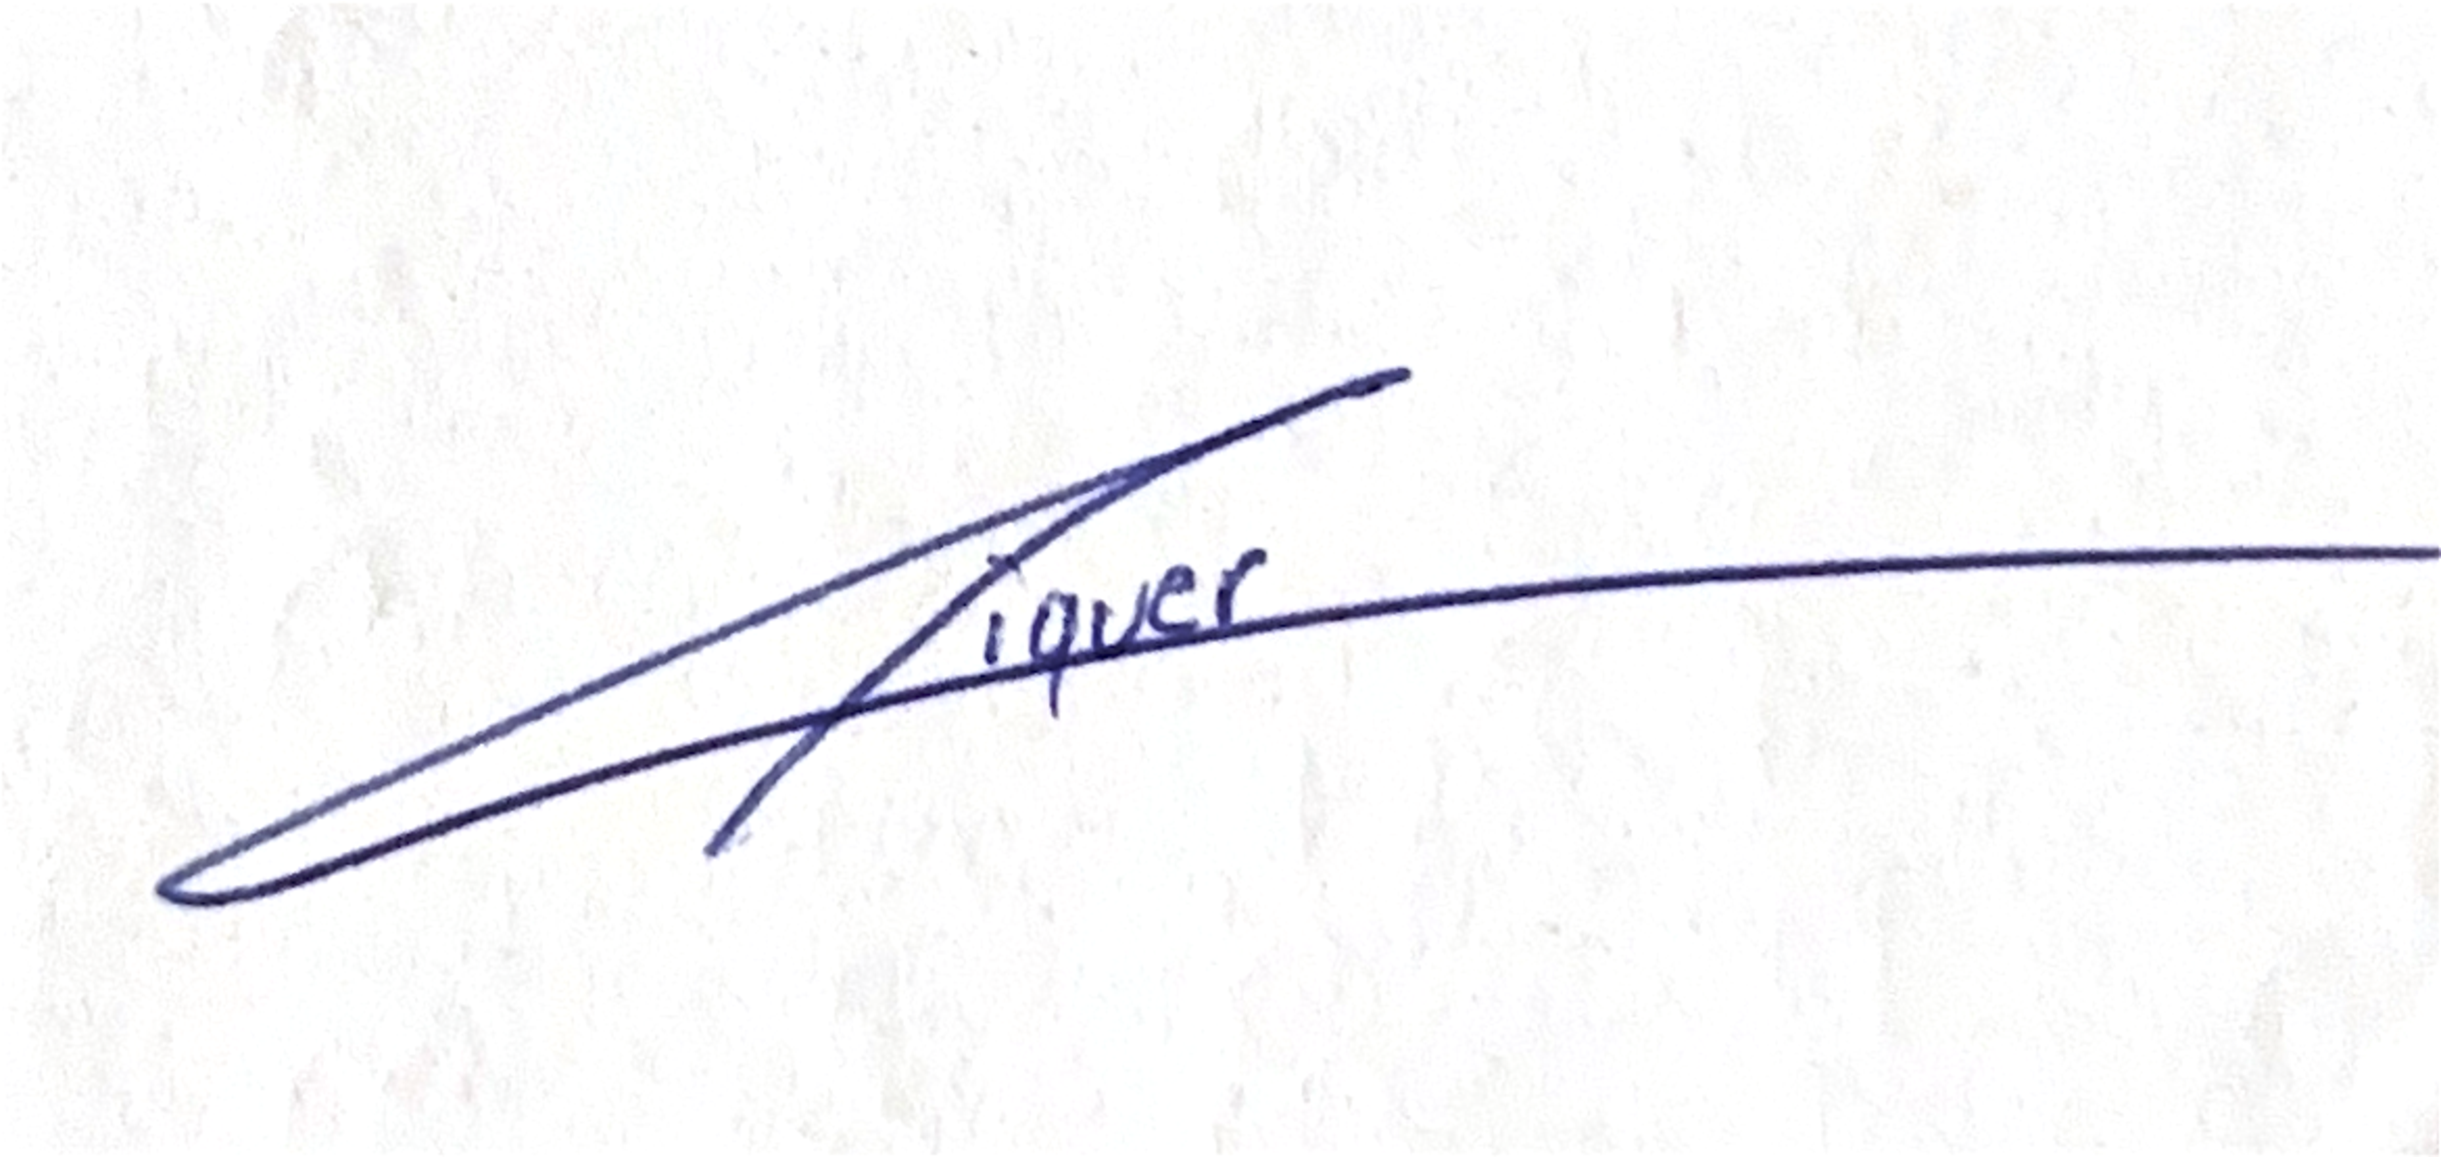
\includegraphics[height=1.8cm, trim=200 150 100 150, clip]{figs/firma}}
